% Chapter 3
\chapter{系统设计}

\section{系统总体设计}
本章将介绍基于音频特征建模的哮喘检测系统的实现细节。整个系统的设计架构如图\ref{fig:jiagou}所示:在数据收集阶段,系统收集用户的咳嗽信号后,利用数据增强音频数据,并通过人工音频特征提取和VGGish特征提取。最后将提取到的特征输入SVM分类网络进行分类训练,根据分类指标评估模型的好坏。
\begin{figure}[h]
    \centering
    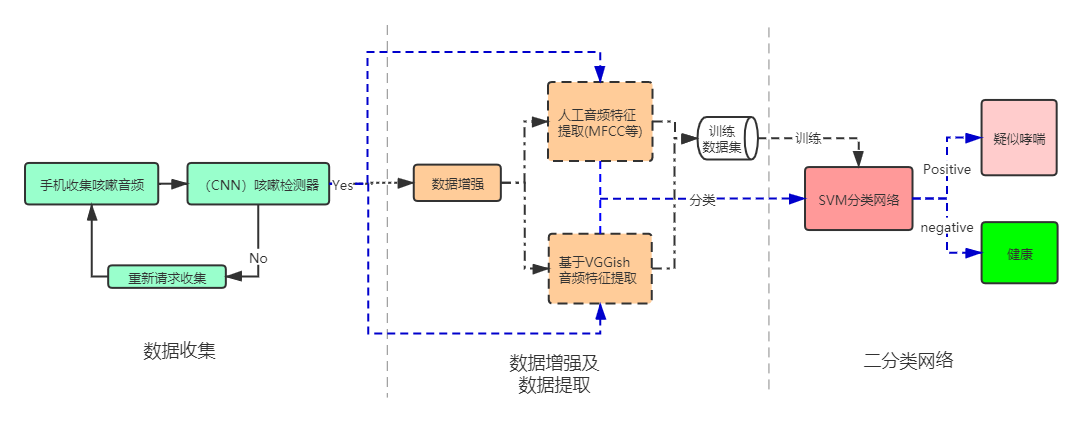
\includegraphics[width=\textwidth]{figures/哮喘检测系统架构.png}
    \caption{哮喘检测系统整体架构}
    \label{fig:jiagou}
\end{figure}

本章主要介绍哮喘检测系统的四个核心部分:(1)利用收集麦克风收集咳嗽音频,并利用CNN神经网络对咳嗽音频的收集结果进行评估;(2)在对咳嗽音频进行音频数据增强后,利用人工处理和VGGish网络进行联合特征提取;(3)SVM分类网络,介绍用于本系统的SVM分类网络架构,简述原因以及分类效果。
\section{原始数据收集及检测}
系统主要基于Android Studio平台搭建了一款收集咳嗽音的手机应用,通过调用手机的麦克风以44.1kHz的采样率对咳嗽音频进行收集,并转化为.wav文件存储到手机本地内存中。但是系统并不能确定原始收集数据是否为咳嗽音频,每一次调用的录音功能都不能保证收集到的数据一定是可用的咳嗽样本。为了使样本满足可用性这一条件,系统需要设计一个简单的CNN网络用于咳嗽样本的检查。

\subsection{咳嗽样本预处理}
根据理论基础中的MFCC理论,系统利用生成咳嗽样本的Mel图用于图像识别分类,处理过程如下:
\begin{enumerate}
    \item 将咳嗽音频重定位至22kHz。
    \item 使用128个Mel成分的三角滤波器对咳嗽音频进行滤波并确定其Mel图。
    \item 调整已经生成的Mel图大小并转化为灰度图,以统一的大小对图像进行缩放并减小图像尺寸,生成\(320\times240\times\)大小的灰度图。
    \item 将生成的图像输入到基于系统的卷积神经网络(CNN)的分类器中,以确定记录的输入声音是否咳嗽
\end{enumerate}

经过系统预处理后的音频图像是一个\(320\times 240 \times 1\)的灰度图,系统用于训练的图展示如图\ref{fig:huidu-image}:其中图\ref{fig:huidu1}为咳嗽音频图像,图\ref{fig:huidu2}和图\ref{fig:huidu3}为其他音源的音频图像。
    \begin{figure}[h]
      \centering
      \begin{subfigure}{0.3\textwidth}
        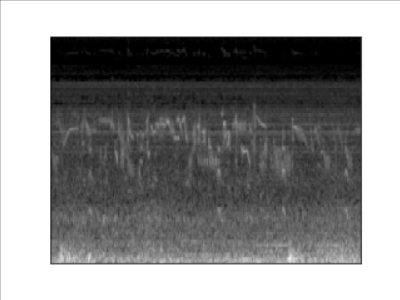
\includegraphics[width=\linewidth]{figures/音频处理1.png}
        \caption{音频灰度图1}
        \label{fig:huidu1}
      \end{subfigure}
      \begin{subfigure}{0.3\textwidth}
        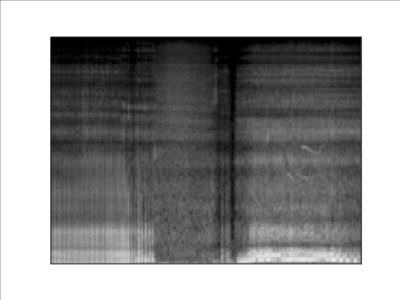
\includegraphics[width=\linewidth]{figures/音频处理2.png}
        \caption{音频灰度图2}
        \label{fig:huidu2}
      \end{subfigure}
        \begin{subfigure}{0.3\textwidth}
        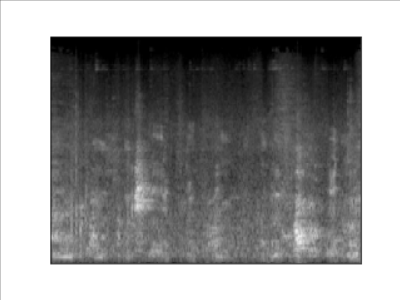
\includegraphics[width=\linewidth]{figures/音频处理3.png}
        \caption{音频灰度图3}
        \label{fig:huidu3}
      \end{subfigure}
      \caption{咳嗽检测训练集样本预处理}
      \label{fig:huidu-image}
    \end{figure}

\subsection{CNN网络结构}
CNN网络的结构设计如图\ref{fig:cnn001},其中包含4个卷积层、3个最大池化层以及1个激活层。最后神经网络生成的2个神经元和softmax激活层用于进行咳嗽与非咳嗽的分类。

\begin{figure}[h]
    \centering
    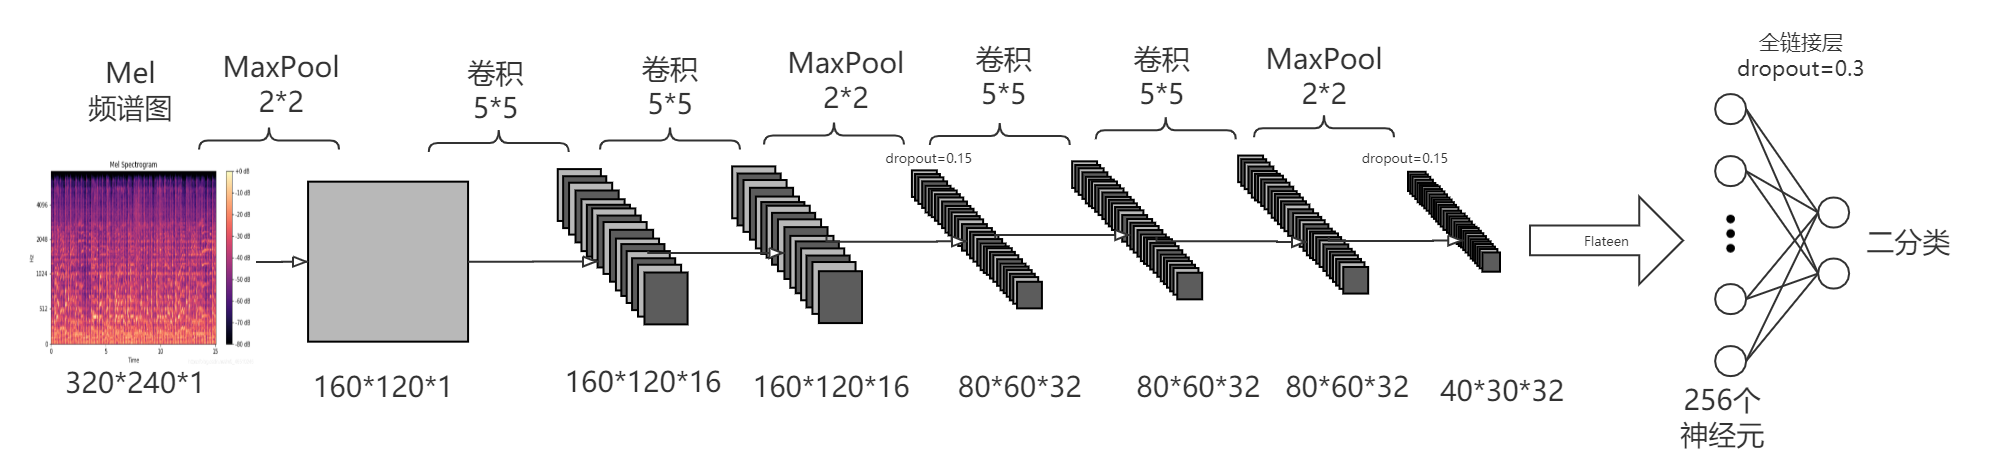
\includegraphics[width=1.1\textwidth]{figures/cnn1.png}
    \caption{咳嗽检测CNN网络}
    \label{fig:cnn001}
\end{figure}

CNN网络的设计思路如下:
\begin{enumerate}
    \item 第一部分是最大池化层。由于输入的Mel光谱图图像尺寸较大,因此在进行下一步之前,首先将其穿过2×2最大池化层以减小整体图像的尺寸,方便进行卷积等特征提取处理。
    \item 第二部分是两个图层块。每个图层包括两个卷积层,并将卷积核大小设置为为5×5,用于提取输入数据的局部特征。其中,第一部分的图层中的卷积层使用了16个过滤器,而第二部分中的两个卷积层使用32个过滤器。系统采用较大的5×5的卷积核是为了减少造成局部特征的过拟合,提高了整体网络的泛化性能与指标。
    \item 第三部分是每个图层块后面的一个2×2的最大池化层以及一个系数为0.15的Dropout层。最大池化层是为了进一步减小图像尺寸,而Dropout层是为了随机让网络某些隐含层节点的权重不对合并进行产生影响,提高整体神经网络的可靠性。
    \item 第四部分是一个完全连接层。系统将从这4个卷积层中学习到的复杂特征进行展平处理,传递到具有256个神经元的完全连接层,最后利用系数为0.3的Dropout层继续防止过拟合情况的发生。
    \item 最后一部分是2个神经源和softmax激活功能的输出层。通过这层结构系统就可以完成对给定输入的咳嗽与非咳嗽音频进行分类。
\end{enumerate}

同时对于该神经网络系统还有一些实现的细节。在该模型中,系统使用ReLU函数作为所有卷积层的激活函数,并利用Adam优化器优化神经的网络结构\cite{kingman2015adam}以及使用交叉熵损失函数作为卷积网络的损失函数。

\section{特征提取}
由于本文使用的数据量较小,系统将采用基于特征的机器学习来提取音频信号的特征向量。系统实现了传统的手工设计特征和迁移学习两种不同的特征提取方法,并使用主成分分析法对系统所有提取到的特征进行降维处理。

\subsection{手工设计特征}
对于咳嗽音频
接下来系统将指明本文挑选的特征值以及挑选的原因
\begin{enumerate}
    \item \textbf{短时平均过零率(Zero Crossing Rate)}:ZCR是指一定时间内音频波形通过直线y=0的次数。这个给特征值在一定程度上反映了频率的大小。ZCR低的音频一般比较浑浊,而ZCR高的音频则比较清澈,因此短时平均过零率用于初步分析清晰、浑浊的音频。通过因为短时平均过零率容易受到低频噪音的干扰,为了提高鲁棒性,系统会在处理中添加阈值,即波形穿过阈值的次数被定义为短时平均过零率。计算算法如下:
\begin{algorithm}[h]
    \caption{ ZCR计算} %算法的名字
    \hspace*{0.02in} {\bf Require:}\\%算法的输入, 
    采样率:fs,一段时间的音频信号:f(t),帧长:wlen,帧移:inc,阈值:\(\alpha\)\\
    \hspace*{0.02in} {\bf Ensure:} %算法的结果输出
    \begin{algorithmic}[1]
    \State 消除直流分量  f(t) = f(t)-mean(f(t)) % \State 后写一般语句
    \State 初始化 wlen = 200, inc = 80, count=0, \(\alpha\)=0.05*max(f(t))
    \State 分帧F, 获取帧数fn
    \State \textbf{for} i = 1:fn \textbf{then}
      \State z=F[i]
      \State \textbf{for} i = 1:(wlen-1) \textbf{then}\\
                \textbf{if} z(j)*z(j+1)<\(\alpha\) \textbf{then}\\
                    count++;\\
        \textbf{end}\\
        \textbf{end}\\
    \textbf{end}
    \State \Return count
    \end{algorithmic}
\end{algorithm}
    \item \textbf{短时音频能量}:短时音频能量是音频信号相应的帧长归一化的振幅值的平方和,依然是用来分辨清澈和浑浊音频的的指标,在时刻T,其计算公式如下:
    \begin{equation}
        E_n = \sum_{m=t-(N-1)}^{t} F[m]^2
    \end{equation}
    \item \textbf{能量熵}:系统将子帧归一化后取其能量的熵,用来度量音频中突变音的发生。
    \item \textbf{共振峰频率}:共振峰是由人声道的共振引起的频谱整形。
    \item
    \textbf{峰度}:峰度是对实值随机变量的概率分布的右部分的度量。
    \item
    \textbf{RMS能量}:RMS能量是信号功率的短时傅里叶变换幅度的均方根,用于表征信号中的能量大小。
    \item
    \textbf{频谱质心}:功率谱图每帧功率的平均值(即质心)。
    \item
    \textbf{截止频率}:功率谱图的中心频率,以便此帧中至少85\%的频谱能量包含在该值及以下。
    \item
    \textbf{MFCC}:MFCC反映了频谱的轮廓,系统基于非线性Mel尺度上对数功率谱的线性余弦变换,从短期功率谱获得Mel频率倒谱系数。系统使用前13个分量的值。
    \item
    \textbf{\(\Delta\)-MFCC}:MFCC的时间微分
    \item
    \textbf{\(\Delta^2\)-MFCC}:MFCC增量的微分(加速度系数)
\end{enumerate}

对于产生的具有时间性质的特征(如:均方根能量、频谱质心、截至频率和MFCC的所有变体),系统提取了一些统计特征,以便捕捉超出平均值的分布。包括:平均值,中位数,均方根,最大值,最小值,1/4位数和3/4位数,四分位的间距,标准差,偏度,峰度。总共有477个手工设计特性,包括3个段级特性、4个由其统计数据表示的帧级特性和3个MFCC的特征,每个组件由其统计数据表示(3+4)× 11 + 3 × 13× 11 = 516。
\subsection{迁移学习特征}
除了手工设计的特征外,系统还使用VGGish来自动提取音频特征[15]。
VGGish是一个卷积神经网络,主要用于基于原始音频输入的音频分类。VGGish是使用大型YouTube数据集进行了训练的模型,并公开发布了学习到的模型参数。因此本系统将其用作特征提取器,将原始音频波形转换为嵌入(特征),然后将其传递以训练SVM分类器。具体训练方法如下:
\begin{enumerate}
    \item 将音频重采样为 16kHz 单声道,
    \item 使用 25ms 的帧长、10ms 的帧移,以及 Hann 窗口对咳嗽音频进行分帧,切割为0.96s的非重叠子帧
    \item 对每一帧做傅里叶变换,然后利用信号幅值计算声谱图
    \item 通过将声谱映射到 64 阶 mel 滤波器组中计算 mel 声谱,并对声谱图取对数能量
    \item 模型每0.96秒返回128维特征向量,将整个线段的均值和标准差作为最终特征,尺寸为256(128×2)
\end{enumerate}

需要注意的是由于VGGish仅基于频谱图输入,因此时域中的一些重要特征可能会在特征空间中遗漏。

\section{支持向量机}
\subsection{概述}
支持向量机(support vectormachines)是机器学习中最经典的二分类模型。这种分类器提供了一种有监督的学习模型,该模型在训练后得到一个最大分离两类的超平面决策边界。

一般来说,为了处理非线性可分的数据,SVM可以加入适当的核,将原始特征空间转换为高维空间,在高维空间中,转换后的特征成为线性可分的(见图4的解释说明)。形式上,选择决策超平面\(w^Tφ(x) + b = 0\)(其中φ(x)表示变换特征空间中的一个点向量,φ为核函数,w为权向量,b为偏差)来最大化整体分离。相当于最大化公式\ref{eq:svm}
\begin{equation}
    \label{eq:svm}
    \sum_{i=1}^n \alpha_i -0.5\sum_{i=1}^n \alpha_i \alpha_j y_i y_j K(x_i,x_j)
\end{equation}

其中\(a_i \ge 0,i=1,2,...n\),且\(\sum_{i=1}^n\alpha_i y_i=0\)。对于每一个数据的索引i,\(x_i,y_i\)分别表示特征向量和对应类的标签(+1代表正样本,-1代表负样本),并且K表示核函数,n表示数据集的大小,\(\alpha_i\)代表拉格朗日乘数。

本理论介绍两类支持向量机的分类性能,其中一种向量机的核函数为线性核(即:\(K(x_i, x_j) = x_i^T x_j\)),另一种的核函数是径向基函数(即\(K(x_i,x_j) = exp \frac{|x_i-x_j|^2}{2σ^2})\),这是一种泛在非线性核。

\subsection{性能表现}
为了评估分类性能,SVM参数,即权重向量w和偏差b,在数据子集(训练子集)上进行优化,并针对互补(测试)子集进行验证。准确地说,数据集被划分为训练和测试的子集,这样:(1)他们大小的比率,称为训练-测试比率,这是一个预先分配好的参数;(2)这些子集中健康以及患病的比例也大致于训练-测试比率相同。一般情况下,分类器的性能取决于主观选择的分割条件。为了避免性能分析中这种主观性,通常使用蒙特卡罗交叉验证(MCCV)\cite{2001Monte},如图\ref{fig:MCCV}所示,本文的所有数据集被随机划分大量(5000)次(迭代),并分割比和前面提到的训练-测试比例保持不变。在每一次迭代,SVM参数在训练子集上进行优化,并记录平均训练、测试精度和相应的标准差。
\begin{figure}
    \centering
    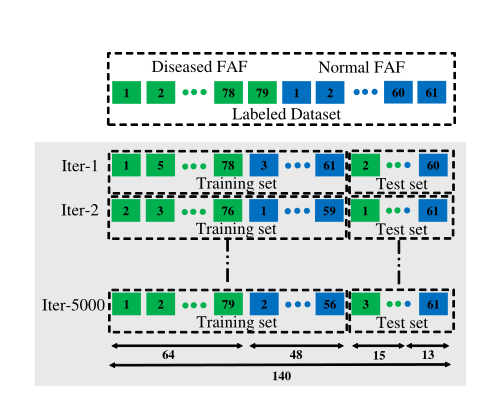
\includegraphics{figures/MCCV.PNG}
    \caption{MCCV方法流程}
    \label{fig:MCCV}
\end{figure}

值得注意的是,训练精度表明了当前模型对可见数据的分类性能,而测试精度表明,对于不可见数据,平均测试精度高的分类器具有实际意义。此外,低标准差(该情况表明在随机分区上的低可变性,从而表明系统的健壮性)是可取的。并且通过计算了超过5000次迭代的平均混淆矩阵,系统提供了健康类和疾病类的每个类条件检测概率。最终实验环节实验组训练和观察了SVM分类器不同的训练-测试比率对SVM性能的影响。